%===========================================================
% This is the thesis template for the Statistics major at
% Amherst College. Brittney E. Bailey (bebailey@amherst.edu)
% adapted this template from the Reed College LaTeX thesis
% template in January 2019 with major updates in April 2020.
% Please send any comments/suggestions: bebailey@amherst.edu

% Most of the work for the original document class was done
% by Sam Noble (SN), as well as this template. Later comments
% etc. by Ben Salzberg (BTS). Additional restructuring and
% APA support by Jess Youngberg (JY). Email: cus@reed.edu
%===========================================================

\documentclass[12pt, twoside]{amherstthesis}
\usepackage{graphicx,latexsym}
\usepackage{amsmath}
\usepackage{amssymb,amsthm}
\usepackage{longtable,booktabs} %setspace loaded in .cls
\usepackage[hyphens]{url}
\usepackage{hyperref}
\usepackage{lmodern}
\usepackage{float}
\floatplacement{figure}{H}
\usepackage{rotating}
\usepackage{fancyvrb}
% User-added packages:
% End user-added packages

%===========================================================
% BIBLIOGRAPHY FORMATTING

% Next line commented out by CII
%%% \usepackage{natbib}
% Comment out the natbib line above and uncomment the
% following two lines to use the new biblatex-chicago style,
% for Chicago A. Also make some changes at the end where the
% bibliography is included.
%\usepackage{biblatex-chicago}
%\bibliography{thesis}


%===========================================================
% HYPERLINK FORMATTING

% Added by CII (Thanks, Hadley!)
% Use ref for internal links
\renewcommand{\hyperref}[2][???]{\autoref{#1}}
\def\chapterautorefname{Chapter}
\def\sectionautorefname{Section}
\def\subsectionautorefname{Subsection}
% End of CII addition
\usepackage{xcolor}
\hypersetup{
    colorlinks,
    linkcolor={red!50!black},
    citecolor={blue!50!black},
    urlcolor={blue!80!black}
}

%===========================================================
% CAPTION FORMATTING

% Added by CII
\usepackage{caption}
\captionsetup{width=5in}
% End of CII addition

%===========================================================
% TITLE FORMATTING

\renewcommand{\contentsname}{Table of Contents}

\usepackage{titlesec}
%%%%%%%%
% How to use titlesec:
% \titleformat{⟨command⟩}[⟨shape⟩]{⟨format⟩}{⟨label⟩}{⟨sep⟩}
%  {⟨before-code⟩}[⟨after-code⟩]
%%%%%%%%

\titleformat{\chapter}[hang]
{\normalfont%
    \Large% %change this size to your needs for the first line
    \bfseries}{\chaptertitlename\ \thechapter}{1em}{%
      %change this size to your needs for the second line
    }[]

\titleformat{\section}[hang]
{\normalfont%
    \large % %change this size to your needs for the first line
    \bfseries}{\thesection}{1em}{%
     %change this size to your needs for the second line
    }[]

\titleformat{\subsection}[hang]
{\normalfont%
    \normalsize % %change this size to your needs for the first line
    \bfseries}{\thesubsection}{1em}{%
     %change this size to your needs for the second line
    }[]

% \titleformat{\section}[display]
% {\normalfont%
%     \large% %change this size to your needs for the first line
%     \bfseries}{\chaptertitlename\ \thechapter}{20pt}{%
%     \normalsize %change this size to your needs for the second line
%     }


%===========================================================
% DOCUMENT FONT

% \usepackage{times}
% other fonts available eg: times, bookman, charter, palatino


%===========================================================
% PASSING FORMATS FROM RMD --> LATEX

%%%%%%%%
% NOTE: Dollar signs pass parameters between YAML inputs
% in index.Rmd and LaTeX
%%%%%%%%

\Abstract{
The abstract should be a short summary of your thesis work. A paragraph is usually sufficient here.
}

\Acknowledgments{
Use this space to thank those who have helped you in the thesis process (professors, staff, friends, family, etc.). If you had special funding to conduct your thesis work, that should be acknowledged here as well.
}

\Dedication{

}

\Preface{

}

% Formatting R code display
% Syntax highlighting #22

% Formatting R code: set baselinestretch = 1.5 for double-spacing
\DefineVerbatimEnvironment{Highlighting}{Verbatim}{
  baselinestretch = 1,
  commandchars=\\\{\}}

% Formatting R output display: set baselinestretch = 1.5 for double-spacing
\DefineVerbatimEnvironment{verbatim}{Verbatim}{
  baselinestretch = 1,
  % indent from left margin
  xleftmargin = 1mm,
  % vertical grey bar on left side of R output
  frame = leftline,
  framesep = 0pt,
  framerule = 1.5mm, rulecolor = \color{black!15}
  }

\title{My amazing title}
\author{Tony Ni}
\date{April DD, 20YY}
\division{}
\advisor{Brittney Bailey}
% for second advisor
\institution{Amherst College}
\degree{Bachelor of Arts}
\department{Mathematics and Statistics}

% Fix from pandoc about cslreferences?
% https://github.com/mpark/wg21/issues/54
\newlength{\cslhangindent}
\setlength{\cslhangindent}{1.5em}
\newenvironment{cslreferences}%
  {\setlength{\parindent}{0pt}%
  \everypar{\setlength{\hangindent}{\cslhangindent}}\ignorespaces}%
  {\par}

% Added by CII
%%% Copied from knitr
%% maxwidth is the original width if it's less than linewidth
%% otherwise use linewidth (to make sure the graphics do not exceed the margin)
\makeatletter
\def\maxwidth{ %
  \ifdim\Gin@nat@width>\linewidth
    \linewidth
  \else
    \Gin@nat@width
  \fi
}
\makeatother

% ===========================================
% DOCUMENT SPACING

\setlength{\parskip}{0pt}
% Added by CII

\providecommand{\tightlist}{%
  \setlength{\itemsep}{0pt}\setlength{\parskip}{0pt}}


% ===========================================
% ===========================================
% ===========================================
\begin{document}

\doublespace
% Everything below added by CII
  \maketitle

\frontmatter % this stuff will be roman-numbered
\pagenumbering{roman}
\pagestyle{fancyplain}
%\pagestyle{fancy} % this removes page numbers from the frontmatter

  \begin{abstract}
    The abstract should be a short summary of your thesis work. A paragraph is usually sufficient here.
  \end{abstract}
  \begin{acknowledgments}
    Use this space to thank those who have helped you in the thesis process (professors, staff, friends, family, etc.). If you had special funding to conduct your thesis work, that should be acknowledged here as well.
  \end{acknowledgments}

  \hypersetup{linkcolor=black}
  \setcounter{tocdepth}{2}
  \tableofcontents

  \addcontentsline{toc}{chapter}{List of Tables}\listoftables

  \addcontentsline{toc}{chapter}{List of Figures}\listoffigures


\mainmatter % here the regular arabic numbering starts
\pagenumbering{arabic}
\pagestyle{fancyplain} % turns page numbering back on

\hypertarget{intro}{%
\chapter{Introduction}\label{intro}}

\hypertarget{background}{%
\section{Background}\label{background}}

Coal is one of the most dangerous combustible fuels which is being burned in all across the world as one of the largest methods of obtaining energy. Yet, although it is a fossil fuel which is naturally abundant and easy to utilize, it is comprised of a long list of dangerous chemicals including -- but not limited to: arsenic, radium, boron, and a large list of other chemicals which prove to be dangerous to humans and animals alike. (Kelderman et al., 2019)

Power plants produce electricity by burning this coal, and as a result of how prevalent it is within the US - over 100 million tons of coal ash are produced every year. This side-product as a result of the coal combustion is often disposed by directly being dumped into landfills and waste ponds. (Kelderman et al., 2019)

Only recently have these complaints and lawsuits regarding the disposing practices made by non-profit environmental organizations been heard. Due to the onslaught of pressure put on the Environmental Protection Agency -- the Coal Ash Rule was bor in 2015. (Kelderman et al., 2019)

This rule has forced over 265 coal power plants -- about 3/4 of all coal power plants in the US - to make data regarding chemical concentrations publicly available to the general population. (Kelderman et al., 2019)

In their analysis using this data, the Environmental Integrity Project -- a non-profit organization dedicated to issues involving environmental justice have concluded that essentially all groundwater under coal plants are contaminated. (Kelderman et al., 2019)

However, is this really the case? There are many naturally occurring chemicals existing in groundwater as as such, perhaps their claims are overstated.
\begin{figure}

{\centering 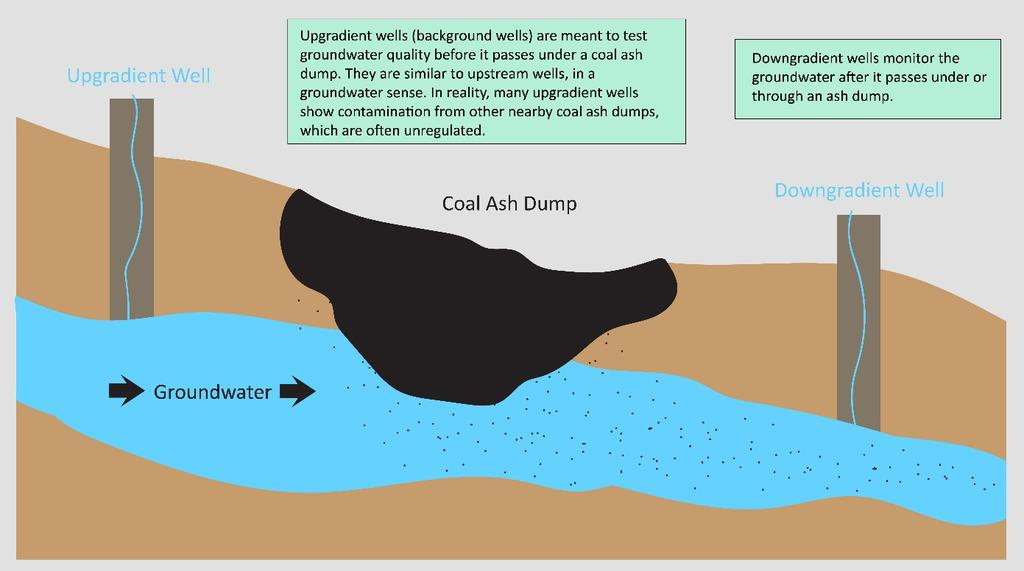
\includegraphics[width=1\linewidth]{figures/upgradientdowngradient} 

}

\caption{Difference Between Upgradient and Downgradient Wells}\label{fig:upgradientdowngradient}
\end{figure}
Typically in a coal ash plant, there exists two types of wells: upgradient wells and downgradient wells. These wells are essential to measure the amount of contamination being caused by coal ash. Upgradient wells, also known as background wells, measures the concentrations of chemicals in groundwater before it passes through an coal ash dump. Conversely, downgradient wells measure the concentrations of chemicals in groundwater after it passes through a coal ash dump.
\begin{itemize}
\tightlist
\item
  ``80\% of the US population is served by 14\% of the utilities,'' so if something were to get into the water distribution system, it can easily spread amongst the US population which is why contamination in water services is so important. (Byer \& Carlson, 2019)
\end{itemize}
With this information, typically -- one estimates the amount of chemical contamination caused by a coal as dump by subtracting the upgradient concentration from the downgradient concentration of a chemical (downgradient concentration - upgradient concentration).

However, due to the lack of proper reporting guidelines prior to the enactment of the Coal Ash Rule, we believe that there may be retired or even unregulated upgradient wells which can cause the concentrations of chemicals being recorded from these upgradient wells to be inaccurate or even completely wrong.

Our end goal remains the same as the EIP: to identify contaminated groundwater in coal plants -- but to attempt to find a way to effectively correct the improper/inaccurate values resulting from LOD errors and other factors which the EIP may not have considered.

The limit of detection problem stems from the measuring devices' inability to obtain chemical concentrations smaller than a certain threshold amount, thus affecting the measurements recorded.

Our plan is to utilize bootstrapping and imputation techniques to correct for these measurements by accounting for the innate contamination which may be caused by factors such as retired and unregulated wells that were mentioned before.

\hypertarget{data}{%
\section{Data}\label{data}}

\hypertarget{coalashrule}{%
\subsection{Coal Ash Rule}\label{coalashrule}}

A large coal ash spill at the Tennessee Valley Authority (TVA) which occured on December 22, 2008 in Kingston, TN -- prompted the Environmental Protection Agency (EPA) to propose a set of standardized regulations and procedures to address the concerns regarding coal ash plants nationwide in the US. (Environmental Protection Agency, 2020)

This was known as the Coal Ash Rule, passed on December 19, 2014. (Environmental Protection Agency, 2020)

Changes were made to the Coal Ash Rule over the years in the form of `amendments,' one of which made required facility information and data to be made publicaly available to the public (April 15, 2015 rule change) (Environmental Protection Agency, 2020)

\hypertarget{source-of-data}{%
\subsection{Source of Data}\label{source-of-data}}

The data used in the study are from the results published in ``Annual Groundwater Monitoring and Corrective Action Reports'' which were made available to the public in March 2018 as a result of the Coal Ash Rule. (Environmental Integrity Project, 2020)

These reports are in PDF format and are thousands of pages long, which makes it difficult for individuals to look through the data in a meaningful way. (Environmental Integrity Project, 2020)

The EIP obtained the data from an online, publicly available database containing groundwater monitoring results from the first ``Annual Groundwater Monitoring and Corrective Action Reports'' in 2018 which was collected from coal plants and coal ash dumps under the Coal Ash Rule (Environmental Integrity Project, 2020)

They wrangled the data into a more accessible machine-readable format which contains information from over 443 annual groundwater monitoring reports posted by 265 coal ash plants, which is downloadable from the EIP's website. (Environmental Integrity Project, 2020)

\newpage

\hypertarget{variables}{%
\subsection{Variables}\label{variables}}

The dataset contains information regarding chemical concentrations at coal plants. A coal plant consists of multiple disposal areas for the coal ash that it produces. At each disposal area, there are specific locations that groundwater is being measured, known as wells which represent an observation in the dataset. There are two types of wells -- upgradient and downgradient wells. The variables consist of information regarding the specific chemical concentrations of each well. From the 19 different contaminants (antimony, arsenic, boron, etc.) a major problem is that some wells only have measurements for certain chemicals and don't have them for others.

\hypertarget{plan-of-action}{%
\subsection{Plan of Action}\label{plan-of-action}}

Within the report, the EIP mentions certain restrictions within the data that have caused their data to potentially be inaccurate (specifically, with limit of detection problems, and a large amount of missing chemical data). The limit of detection problem comes when measuring devices used to measure chemical concentrations are unable to detect below a certain threshold, causing large numbers of observations to have duplicate, wrong values -- which can cause for misguided analysis.The other issue is less guided/formed, but for brevity, we think that a lot of the issues in the data comes from the potential possibility of contamination during data collection from investigators from non coal-ash sources. This may include things like: retired/unregulated wells which are old and have chemicals leaking into the groundwater, mismanagement in measuring, etc.My project hopes to work with methods on handling this missing data -- alongside investing potential uses of bootstrapping and other resampling methods (potentially?) in order to try to come up with a more statistically accurate and sound result by looking to assuage the problems that the EIP faced in their analysis. Specifically, to find a way to split up the data into ''uncontaminated'' and ''contaminated'' wells in order to find the natural distribution of chemicals in each -- and doing to so in the face of data corrupted by LOD problems and inaccuracies. I'm hoping to apply and compare different ways of altering the data to account for these myriad of issues in order to look for more salient findings that the EIP might have missed or if not, to see if improvements can be made regarding the way that contaminated coal ash wells are being identified.

\hypertarget{methodology}{%
\chapter{Methodology}\label{methodology}}

The concept of missing data is ubiquitous within academic disciplines and which frequently complicates any types of real-world studies. Missing data will be defined within this thesis as \emph{occurences within a dataset where there is no value stored for a variable in the observation of interest}. As most studies often utilize data collected through mediums such as surveys, questionnaires, or field research, missing data is an unavoidable problem. Missing data hinders one's ability to work with and analyze the phenomena at hand, as data is often the basis of all studies. One of the most glaring issues with missingness is how it can introduce bias within an analysis, which can more often than not, invalidate a study if not accounted for and handled properly.

This thesis will go into a more specific instance of missing data known as censoring, which is \emph{the condition when one has only partial information regarding the values of a measurement within a dataset}. We will introduce and define the three types of censored data, challenges with the reporting of censored data, alongside a discussion on common statistical approaches to handling censored data.

\hypertarget{censored_data}{%
\section{Censored Data}\label{censored_data}}

As discussed previously, censored data is a specific type of missingness where one has only partial information regarding the values of a measurement in a dataset. There are many types of censoring which can occur, but three main ones which are the most common: right censoring, interval censoring, and left censoring.

\hypertarget{right}{%
\subsection{Right Censoring}\label{right}}

Right censoring is a specific instance in which we only know that the true value of a data point lies above a certain threshold, but it is unknown by how much. Suppose a study on income and mortality is conducted with the variable of interest, \(T\), being the time measured from the start of the study to the death of the participant. The study has a duration of 5 years, in which participants are expected to submit a form regarding their annual income. The value for the participant would be considered to be right-censored if at any point during the study, they failed to follow-up, or if the participant was still alive at the conclusion of the 10 year study. In this design study, several possibilities can occur, illustrated in figure blah.
\begin{figure}

{\centering 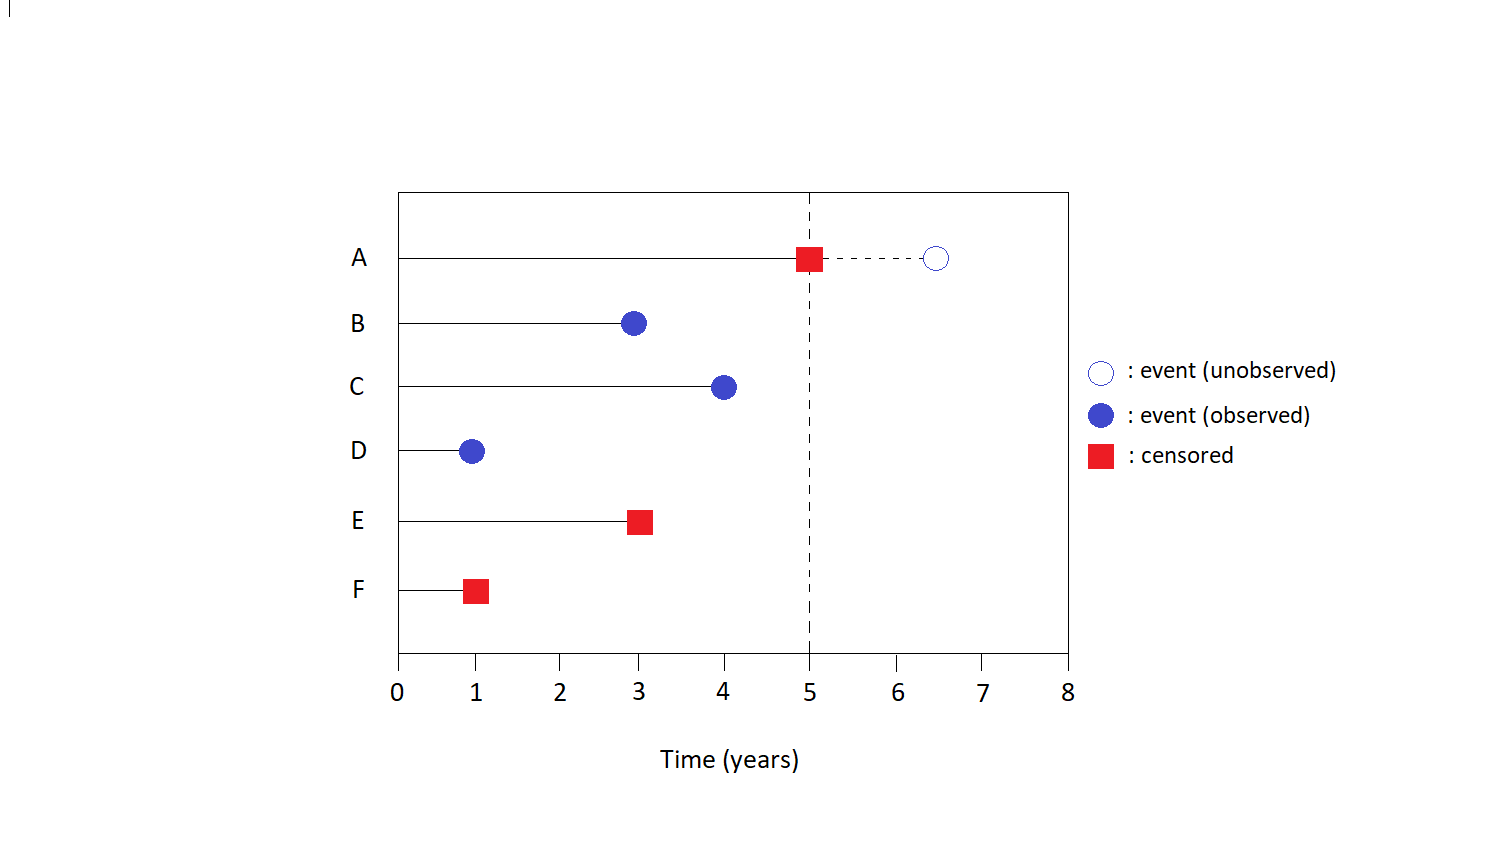
\includegraphics[width=1\linewidth]{figures/right_censoring_example} 

}

\caption{Right Censoring Example}\label{fig:rightcensoringexample}
\end{figure}
If the individual passes to the termination of the study, the only information we have is \(T > 5\).

If an individual passes away at some point, \(t_i\) during the study, then \(T = t_i\).

Suppose an individual stopped submitting a form during the third year of the study. As we have no information about whether or not if they died or simply did not submit their form, all we know is that the individual died/will die at some point after year three of the study. In this instance, \(T > 3\).

Right censoring is the most common type of censoring and can often be found in clinical trial studies, mortality studies, and other forms of surival analyses.

\hypertarget{left}{%
\subsection{Left Censoring}\label{left}}
\begin{figure}

{\centering 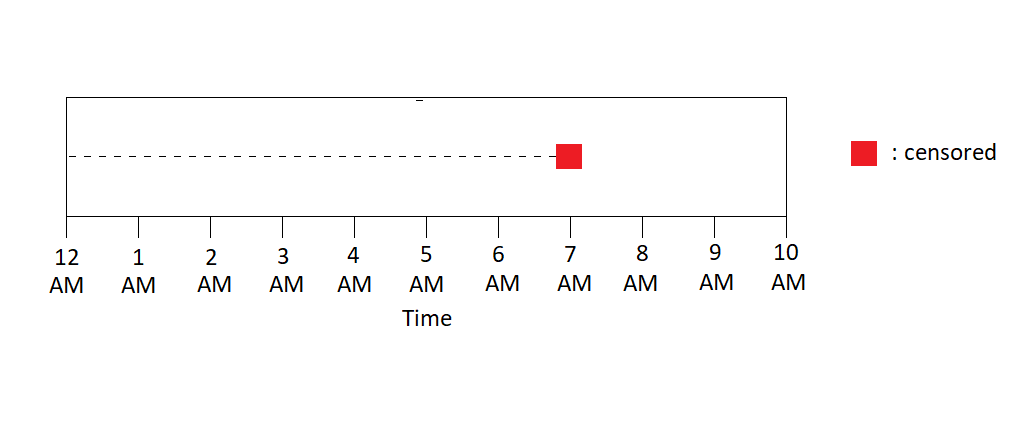
\includegraphics[width=1\linewidth]{figures/left_censoring_example_fix} 

}

\caption{Left Censoring Example}\label{fig:leftcensoringexample}
\end{figure}
In contrast with right censoring, left censoring is a specific instance of censoring in which we only know that the true value of a data point falls below a certain threshold which we call the \emph{limit of detection} (LOD).

To understand this concept better, consider the following example. Imagine a scenario in which you are attempting to estimate the time at which the sun rises each morning. You plan to wake up every morning far before the sun rises, but on the first day of the study, you oversleep and wake up at 7:00 A.M. with the sun already out. We now have an instance of left-censored data. We want to know the time at which the sun rose, but all we have is an upper limit (7:00 A.M.).

Left censoring is commonly found in environmental, water quality, and chemical-related research, where the focus is on the concentration of an analyte. Due to limitations on measuring instruments, left censored data are commonly found in these types of studies.

\hypertarget{interval}{%
\subsection{Interval Censoring}\label{interval}}
\begin{figure}

{\centering 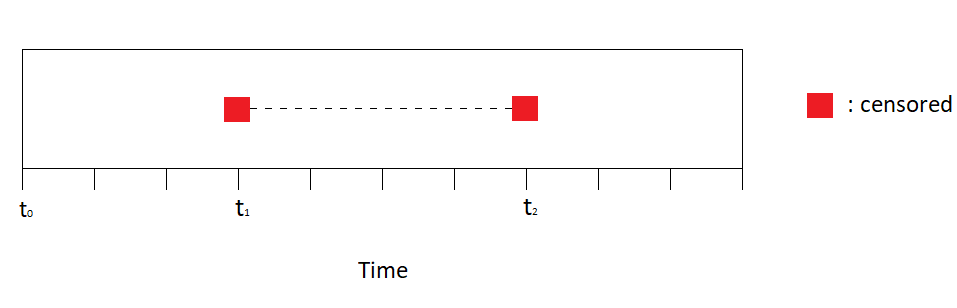
\includegraphics[width=1\linewidth]{figures/interval_censoring_example_fix} 

}

\caption{Interval Censoring Example}\label{fig:intervalcensoringexample}
\end{figure}
Interval censoring is another form of censoring in which the random variable of interest is known to be between an interval of two values. Considering a random variable \(T\), which denotes the survival time of interest, if interval censoring is at hand, we can denote the interval containing \(T\) to be \(I = [L, R]\), with \(L\) being the beginning of the interval and \(R\) being the end of the interval.

Left and right censoring are special cases of interval censoring. In the case of left censoring, \(L = 0\); and conversely in the case of right censoring, \(R = \infty\).

To conceptualize interval censoring, we can consider a example study on virus testing, in which participants get their blood drawn in order to detect whether or not if they test positive for the virus or not. The random variable in question is \(T\), which represents the exact timepoint at which the subject contracted the virus. If an individual was first tested at time \(t_1\) and tested negative, but was tested again at a later time \(t_2\) and tested positive, the specific time \(t\) at which the subject contracted the virus is unknown. All we know is that it lies somewhere between the interval is \(I = [t_1, t_2]\), but not the exact time at which they contracted it.

There are a myriad of types of censoring which can be discussed, however the focus of my thesis deals specifically with the challenges of reporting these values alongside methods of handling left-censored data.

\hypertarget{challenges}{%
\section{Challenges of Reporting Censored Data}\label{challenges}}

{[}CURRENTLY WORKING ON REORGANIZING HERE{]}

There is no universal reporting practice for values below the LOD which can lead to confusion amongst researchers. The lack of standardization makes it difficult to distinguish LOD values with uncensored values. This can lead to LOD values unintentionally being overlooked, causing faulty analysis or conclusions which are heavily flawed.

In a study involving the precision of lead measurements near concentrations of the limit of detection, Berthouex (1993), discusses this disparity in practice within chemists and their labs and describe in the following list as:
\begin{enumerate}
  \item Reporting the trace, a chemical whose average concentration is less than 100 $\mu g$
  \item Reporting  the letters ND, which stand for "not detected"
  \item Reporting the numerical LOD value itself
  \item Reporting the "less than" value, which is the numerical LOD preceded by a "<"
  \item Reporting some value between 0 and the LOD, such as one-half the LOD value
  \item Reporting the actual measured concentration, even if it falls below the LOD
  \item Reporting the actual measured concentration, followed by (LOD)
  \item Reporting the actual measured concentration with a precision ($\pm$) statement
\end{enumerate}
The latter three methods are the best {[}FIND PAPER BY Gilbert, 1987; Hunt and Wilson, 1986; and Rhodes, 1981 -- backtrace through berthouex when time allows?{]}.

Berthouex discusses the prevalence in regards to the practice of censoring data by reporting only values which are above the detection limit and discarding those which fail to yield quantifiable results. He discourages this practice and instead suggests the reporting the numeric values of measurements, even when those values are below the limit of detection. (Berthouex, 1993)

\hypertarget{Approaches}{%
\section{Approaches}\label{Approaches}}

{[}START HERE{]}

It is important to note that the values below the LOD still contain information, specifically that the values is between the lower bound value (if it exists) and the LOD (Chen et al., 2011). As such, there are a variety of statistical treatments to handle censored data which have been popularized in the statistical literature which will be discussed within this section.

Omission involves the deletion of data points which are deemed to be invalid, as a result of left-censoring or any other deficiencies in the data. This is also more commonly known as \emph{complete-case analysis}, in which statistical analysis is conducted while only considering the observations which have no missing data on the variables of interest, and excluding the observations with missing values (May, 2012). May argues against this approach and claims that the loss of information from discarding data and the inflation of standard errors of estimates (when discussing missingness in a regression context) will invariably be inflated as a result of the decreased sample size. The advantages of omission lies in its ease of implementation. {[}WHAT SORT OF USEFUL INFORMATION IS DISCARDED, INCLUDE HERE, omitting is a valid method which is used by default in a lot of statistical software, when should care be used?{]}

Apart from complete-case analysis, which is of course the most natural idea which pops up in our minds when discussing topics involving missingness and censoring. Over the past century, a myriad of methods to deal with censoring have been developed to counter this issue -- some more statistically sound than others. Some of the most common methods to estimate descriptive statistics involving censored data include but are not limited to: substitution, maximum likelihood estimation, Kaplan-Meier, regression on order statistics, and of course distributional based multiple imputation methods (Lafleur et al., 2011).

\hypertarget{Substitution}{%
\subsection{Substitution Approach}\label{Substitution}}

Often condemned in papers, and rightly so, as a statistically unsound method to handle censored data, substitution methods are unfortunately ubiquitous in many fields outside of statistics as a way to handle censored data sets, often being cited in environmental science papers as an appropriate (and even recommended) method to work with left-censored chemical concentration data (Canales, 2018).

In analytical chemistry, a limit of detection is defined as:

\[LOD = \mu_{blank} + K\sigma_{blank}\]
where the distribution of the blank is assumed to be Gaussian, with mean \(\mu_{blank}\), standard deviation \(\sigma_{blank}\), and K representing a ``definition-specific constant,'' which is usually between the range 2.0 to 3.0. Ideally the blank will contain as little of the analyte of interest as possible, as it serves as the control and the basis as to which samples are being compared to. With a K = 3, it is to be expected that around 99.7\% of the observations from a blank sample will be below the limit of detection as per the empirical rule for a Gaussian distribution (May, 2012).

Once the LOD is determined for the study, the substitution method simply involves imputing in a replacement value in lieu of the censored data point.

This replacement value used may differ between studies but common values include: \(\frac{LOD}{2}, \frac{LOD}{\sqrt2}\), or \(LOD\). Different disciplines have their own suggested ``best,'' replacement value to use (Lee \& Helsel, 2005). Of course there may be more out there, but it must be recognized that the substitution method is a statistically \emph{unsound} technique which are used often in non-rigorous statistical settings due to them being quite easy to implement (Chen et al., 2011).

In a study performed by Glass to investigate the effectiveness of LOD approaches, they used a variety of naive substitution methods from the values listed previously. The investigated substitution enthusiasts' claims of certain replacement values being more apt for certain types of data sets. These proponents of the method claim that the replacement value \(\frac{LOD}{2}\) is useful for data sets in which lots of data are below the LOD or when the data is highly skewed with a geometric standard deviation (a measure of spread commonly used in tandem with log-normal distributions) of 3 or more. On the same note, they claim that the \(\frac{LOD}{\sqrt2}\) is helpful for cases when there are only a few data points below the LOD or when the data is not highly skewed. From Glass' results, it was found that both of these methods are equally unsound in their reasoning and logic as they both introduce large errors and biases regardless of the data set being used (Glass \& Gray, 2001).

\hypertarget{MLE}{%
\subsection{Maximum Likelihood Estimation}\label{MLE}}

Maximum likelihood is a parametric technique which allows us to estimate the parameter values of a distribution/model and one which is useful when encountering censored data.

To give a brief introduction as to the the mechanisms of MLE and how it functions, given a random \emph{i.i.d.} set of random variables \(X_1, X_2,...,X_n\) from distribution \(f(x|\theta)\).

For every observed random sample \(x_1,...,x_n\), we can define the joint density function to be:

\[f(x_1,...,x_n|\theta) = f(x_1|\theta)...f(x_n|\theta) = \prod_{i=1}^{n}f(x_i|\theta)\]
Upon observing the given data, \(f(x_1,...,x_n|\theta)\) becomes a function of \(\theta\) alone, so we obtain a likelihood of:

\[lik(\theta) = f(x_1,...,x_n|\theta)\]
Our goal is to obtain the maximum likelihood estimate (mle) of \(\theta\) which maximizes \(lik(\theta)\), in other words, to obtain a \(\theta\) which makes our observed data the most probable/likely.

As we previously declared our random variables \(X_1, X_2,...,X_n\) to be i.i.d, we can rewrite the likelihood to be a product of the marginal densities:

\[lik(\theta) = \prod_{i=1}^{n} f(x_i|\theta)\]
in which we can then maximize the likelihood to find the best mle of \(\theta\) to best capture our observed data.

Maximum likelihood estimation is widely thought to be optimal, but only if one knows the proposed model and underlying distribution of the dataset in advance, hence its classification as a parametric technique. In a study comparing methods to handling missing data, Canales found that the MLE method underperformed when the data in question was highly skewed, in which overinflated mean squared errors were often obtained (Canales, 2018).

The MLE method we will be utilizing is actually performed by obtaining regression estimates of slope(s) and intercepts through maximum likelihood with censored data. The \texttt{cenmle} function in the \texttt{NADA} package allows the user to specify censored and uncensored data, and uses the LOD as the placeholder. As this method is not an imputation technique, values are not replaced. This method allows us to calculate the summary statistics for the entire data set -- including the censored values.
\begin{itemize}
\tightlist
\item
  Useful slides to refer to here {[}\url{https://www.eurachem.org/images/stories/workshops/2017_10_PT/pdf/contrib/O05-Mancin.pdf}{]}
\end{itemize}
\hypertarget{Kaplan-Meier}{%
\subsection{Kaplan-Meier Estimate Approach}\label{Kaplan-Meier}}

{[}As a phenomenon, censoring is most often discussed in the branch of statistics known as survival analysis, which concerns itself with techniques to analyze a time to an event variable. As their name suggests, these variables measure the time which passes until some sort of event occurs. The type of event being observed need not be related to issues related to mortality, but it is certainly is most commonly employed in the health-care field. These types of events can be as innocuous as the time until device breaks, time until birds migrate away from their homes, or even things like time until an ice cream scoop falls onto the pavement. Regardless of which, all of these scenarios share a common flaw in terms of the possibility of the data being ``censored.''{]} {[}need to fix bracketed into existing paragraph{]}

The Kaplan-Meier method is a common nonparametric technique used to deal with censored data. Originally developed to handle right-censored survival analysis data, an offshoot method in the form of the Reverse Kaplan-Meier Estimator have sprung up as a way to handle left censored data as well (Gillespie et al., 2010). The advantages of the KM method lie in its robustness as a nonparametric method; it performs well with a wide range of distributions. Many recommend its usage for when there are cases of extreme/severe censoring as a result of this {[}Canales2018{]}.

To introduce the concept of the KM-estimator, it is helpful to take a look into its usages in survival analysis studies where the focus is often on a type of ``time to a certain event occurring'', often being cases such time to death, or time to failure.
\begin{itemize}
\tightlist
\item
  {[}INSERT PICTURE OF EXAMPLE SURVIVAL CURVE HERE{]}
\end{itemize}
The KM-estimator is a nonparametric statistic used to estimate the survival curve from the empirical data while accounting for the possibilities of certain values being censored (participants in a mortality study could drop out, die during the study, become unavailable to contact after a certain time, etc.). It does this by assuming that censoring is independent from the event of interest (death) and that survival probabilities remain the same in observations found early in the study and those recruited later in the study {[}CITE PROPERLY \url{https://sphweb.bumc.bu.edu/otlt/mph-modules/bs/bs704_survival/BS704_Survival_print.html}{]}

The KM-estimator when performing an empirical estimation of the survival curve at time \(t\) can be represented by the following equation:

\[\hat{S}(t) = \prod_{\ x_j \le \ t }(1-\frac{d_j}{y_j})\]
where \(x_j\) is the distinct event/death time, \(d_j\) is the number of event/death occurrences at time \(x_j\), and \(y_j\) is the number of followup times (\(t_i\)) that are \(\ge\) \(x_j\) (how many observations in sample survived at least/or past the time \(t_i\)). {[}CITE PROPERLY WHEN TIME ALLOWS \url{https://www.youtube.com/watch?v=NDgn72ynHcM\&t=398s\&ab_channel=mathetal}{]}

Typically, the KM-estimator can only be used to estimate the distribution function of right-censored data, in which a data point is above a certain threshold, but it is unknown by how much. A simple tweak to the typical KM-method yields the reverse Kaplan-Meier approach, which allows for the estimation of the survival curve with left-censored values. This approach follows exactly the same logic as the Kaplan-Meier estimate of the survival curve, except we reverse the censored indicator and event of interest indicator. In other words, our censor is now the event and the event is now censored. This allows us to estimate the distribution function and population percentiles for data containing left-censored values (Gillespie et al., 2010).

For our analysis, we will be using the \texttt{cenfit} function from the \texttt{NADA} package in R to estimate the empirical cumulative distribution function (survival curve) for our left-censored data using the reverse Kaplan-Meier method. Similarly to the MLE method, the KM method is not an imputation method, so we are not replacing censored values with an imputed value, but rather estimating descriptive statistics for the entire dataset -- including the censored concentrations (Canales, 2018).

\hypertarget{ROS}{%
\subsection{Regression on Order Statistics}\label{ROS}}

In between both the parametric nature of the MLE approach and nonparametric of the Kaplan-Meier estimator is the regression on order statistics (also known as ROS) method. As its name suggests, ROS is a semi-parametric method. It assumes that the censored measurements (emphasis on ONLY the censored, this what makes it semi-parametric) in the data comes from a normal or lognormal distribution.

In the ROS method, in order to model the distribution of the censored values, a linear regression model is created by plotting the uncensored observed values (ordered from smallest to largest) vs.~the quantiles (also known as ``order statistics''), which is then used estimate and impute the values of the censored data (Lee \& Helsel, 2005). These imputed values for the censored portions of the data are then combined with the known values of the uncensored bits, which allows for the computation of the descriptive statistics of interest. In summary, ROS imputes the censored data using the estimated parameters from the linear regression model of the uncensored observed values versus their quantiles.

There are of course, some requirements which must hold in order for ROS to be utilized: at minimum, there needs to be at least 3 known values and more than half the values within the data set must be known. As regression is utilized in this method, additional assumptions in the ROS method are shared with those necessary for linear regression to be performed as well. The response variable must be a linear function of the explanatory variable (quantiles). Additionally, the errors should have constant variance (Lee \& Helsel, 2005).

The \texttt{NADA} package contains the function \texttt{ros} which provides an implementation of regression on order statistics which allows us to calculate descriptive statistics for left censored values.

\hypertarget{simulations}{%
\chapter{Simulations}\label{simulations}}

{[}short passage describing what we hope to gain from performing a simulation study{]}

\hypertarget{ademps}{%
\section{ADEMPS}\label{ademps}}

{[}discuss ademps approach to designing a simulation study{]} (Morris, White, \& Crowther, 2019)

\hypertarget{aims}{%
\subsection{Aims}\label{aims}}

\hypertarget{data_generating_mechanisms}{%
\subsection{Data-Generating Mechanisms}\label{data_generating_mechanisms}}

\hypertarget{estimands}{%
\subsection{Estimands}\label{estimands}}

\hypertarget{methods}{%
\subsection{Methods}\label{methods}}

\hypertarget{performance_measures}{%
\subsection{Performance Measures}\label{performance_measures}}

\hypertarget{results}{%
\section{Results}\label{results}}

{[}place figures/tables from results of simulation study here, along with explanation{]}

\hypertarget{discussion}{%
\section{Discussion}\label{discussion}}

{[}discuss findings from the simulation study. are the results expected from knowledge gained from literature search? are they different?

\hypertarget{limitations}{%
\subsection{Limitations}\label{limitations}}

{[}discuss some limitations of the simulation study -- ideas include things such as how simulated data =/= real life data, discuss some limitations, future plans?{]}

\hypertarget{real_data}{%
\section{Study on Real Data}\label{real_data}}

{[}connect back to chapter 1{]}

\hypertarget{conclusion}{%
\chapter{Conclusion}\label{conclusion}}

{[}write a few paragraphss to wrap up entire thesis{]}

\hypertarget{corrections}{%
\chapter*{Corrections}\label{corrections}}
\addcontentsline{toc}{chapter}{Corrections}

A list of corrections after submission to department.

Corrections may be made to the body of the thesis, but every such correction will be acknowledged in a list under the heading ``Corrections,'' along with the statement ``When originally submitted, this honors thesis contained some errors which have been corrected in the current version. Here is a list of the errors that were corrected.'' This list will be given on a sheet or sheets to be appended to the thesis. Corrections to spelling, grammar, or typography may be acknowledged by a general statement such as ``30 spellings were corrected in various places in the thesis, and the notation for definite integral was changed in approximately 10 places.'' However, any correction that affects the meaning of a sentence or paragraph should be described in careful detail. The files samplethesis.tex and samplethesis.pdf show what the ``Corrections'' section should look like. Questions about what should appear in the ``Corrections'' should be directed to the Chair.

\backmatter

\hypertarget{references}{%
\chapter*{References}\label{references}}
\addcontentsline{toc}{chapter}{References}

\noindent

\setlength{\parindent}{-0.20in}
\setlength{\leftskip}{0.20in}
\setlength{\parskip}{8pt}

\hypertarget{refs}{}
\begin{cslreferences}
\leavevmode\hypertarget{ref-Berthouex1993}{}%
Berthouex, P. (1993). A Study of the Precision of Lead Measurements at Concentrations Near the Method Limit of Detection, \emph{65}(5), 620--629.

\leavevmode\hypertarget{ref-Byer2019}{}%
Byer, D., \& Carlson, K. H. (2019). Real-time detection of intentional chemical contamination in the distributional system, \emph{97}(7), 130--133.

\leavevmode\hypertarget{ref-Canales2018}{}%
Canales, R. (2018). Methods for Handling Left-Censored Data in Quantitative Microbial Risk Assessment, \emph{84}(20), 1--10.

\leavevmode\hypertarget{ref-Chen2011}{}%
Chen, H., Quandt, S. A., Grzywacz, J. G., Arcury, T. A., Environmental, S., Perspectives, H., \ldots{} Arcury, T. A. (2011). A Distribution-Based Multiple Imputation Method for Handling Bivariate Pesticide Data with Values below the Limit of Detection, \emph{119}(3), 351--356. \url{http://doi.org/10.1289/ehp.l002124}

\leavevmode\hypertarget{ref-EIP2020}{}%
Environmental Integrity Project. (2020). Coal Ash Groundwater Contamination: Documenting Coal Ash Pollution. Retrieved from \url{https://environmentalintegrity.org/coal-ash-groundwater-contamination/}

\leavevmode\hypertarget{ref-Car2020}{}%
Environmental Protection Agency. (2020). Disposal of Coal Combustion Residuals from Electric Utilities Rulemakings. Retrieved from \url{https://www.epa.gov/coalash/coal-ash-rule}

\leavevmode\hypertarget{ref-Gillespie2010}{}%
Gillespie, B. W., Chen, Q., Reichert, H., Franzblau, A., Lepkowski, J., Adriaens, P., \ldots{} Garabrant, D. H. (2010). Estimating Population Distributions When Some Data Are Below a Limit of Detection by Using a Reverse Kaplan-Meier Estimator. \emph{Epidemiology}, \emph{21}. \url{http://doi.org/10.1097/EDE.0b013e3181ce9fD8}

\leavevmode\hypertarget{ref-Glass2001}{}%
Glass, D. C., \& Gray, C. N. (2001). Estimating mean exposures from censored data: Exposure to benzene in the Australian petroleum industry. \emph{Annals of Occupational Hygiene}, \emph{45}(4), 275--282. \url{http://doi.org/10.1016/S0003-4878(01)00022-9}

\leavevmode\hypertarget{ref-Kelderman2019}{}%
Kelderman, K., Kunstman, B., Roy, H., Sivakumar, N., Mccormick, S., \& Bernhardt, C. (2019). Coal's Poisonous Legacy: Groundwater Contaminated by Coal Ash Across the U.S.

\leavevmode\hypertarget{ref-Lafleur2011}{}%
Lafleur, B., Lee, W., Billhiemer, D., Lockhart, C., Liu, J., \& Merchant, N. (2011). Statistical methods for assays with limits of detection: Serum bile acid as a differentiator between patients with normal colons, adenomas, and colorectal cancer. \emph{Journal of Carcinogenesis}, \emph{10}, 1--8. \url{http://doi.org/10.4103/1477-3163.79681}

\leavevmode\hypertarget{ref-Lee2005}{}%
Lee, L., \& Helsel, D. (2005). Statistical analysis of water-quality data containing multiple detection limits : S-language software for regression on order statistics \$, \emph{31}, 1241--1248. \url{http://doi.org/10.1016/j.cageo.2005.03.012}

\leavevmode\hypertarget{ref-May2012}{}%
May, R. C. (2012). Estimation Methods for Data Subject to Detection Limits, 82.

\leavevmode\hypertarget{ref-Morris2019}{}%
Morris, T. P., White, I. R., \& Crowther, M. J. (2019). Using simulation studies to evaluate statistical methods. \emph{Statistics in Medicine}, \emph{38}(11), 2074--2102. \url{http://doi.org/10.1002/sim.8086}
\end{cslreferences}
% Index?

\end{document}
